\documentclass[10pt]{article}
\usepackage{amsmath,amssymb,mathtools}
\usepackage{graphicx}
\usepackage[font=small]{caption}
\usepackage{float}
\usepackage{geometry}
\usepackage{enumitem}
\geometry{margin=0.75in}
\setlength{\parskip}{0.25em}
\setlength{\parindent}{0pt}
\setlist[enumerate]{leftmargin=*,itemsep=0.15em,topsep=0.15em}
\captionsetup{skip=2pt}

\DeclareMathOperator{\sinc}{sinc}

\begin{document}

\begin{center}
{\LARGE EE 115 Homework 4}\\[0.25em]
Kaushik Vada \quad November 1, 2025
\end{center}

\section*{Problem 1}
Let $m(t) = 2\,\sinc(3t)$ where $t$ is in milliseconds. With the engineering definition $\sinc(x)=\frac{\sin(\pi x)}{\pi x}$, the Fourier transform is
\[
M(f) = \frac{2}{3}\,\mathrm{rect}\!\left(\frac{f}{3}\right),
\]
so the baseband bandwidth is $B = 1.5~\text{kHz}$ and $f_c = 4B = 6~\text{kHz}$. The input to the nonlinear device is $x_{\text{in}}(t)=m(t)+\cos(2\pi f_c t)$, and the device output is
\[
x_{\text{out}}(t)=\alpha x_{\text{in}}^2(t) - \beta x_{\text{in}}(t).
\]

\begin{enumerate}
\item[(a)] The spectrum of $x_{\text{out}}(t)$ contains (i) a low-pass term from $\alpha m^2(t)$, (ii) shifted replicas about $\pm f_c$ from $2\alpha m(t)\allowbreak\cos(2\pi f_c t)$, (iii) spectral lines at $\{0,\pm f_c,\pm 2f_c\}$ from the carrier harmonics, and (iv) the attenuated baseband $-\beta m(t)$ plus the carrier $-\beta\cos(2\pi f_c t)$. Figure~\ref{fig:q1} overlays these pieces.

\begin{figure}[H]
    \centering
    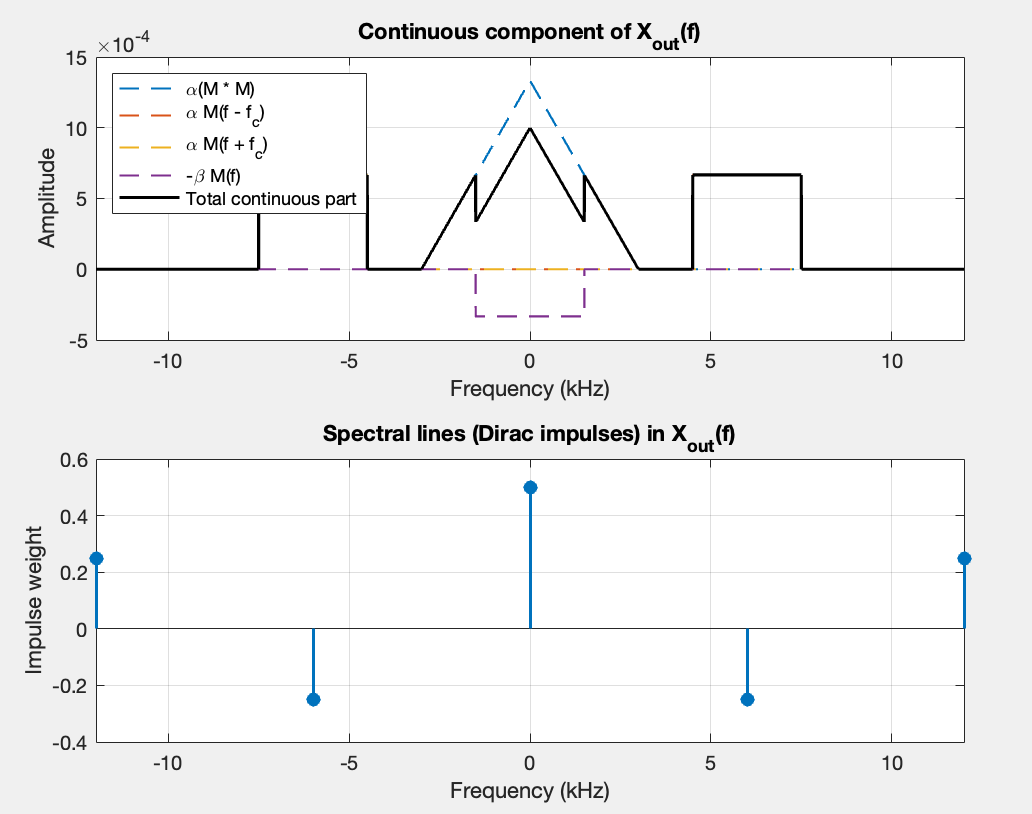
\includegraphics[width=0.7\linewidth]{image/question1.png}
    \caption{Spectral sketch for $X_{\text{out}}(f)$ highlighting the continuous components and the Dirac impulses.}\label{fig:q1}
\end{figure}

\item[(b)] The bandpass filter must extract only the components around $\pm f_c$ while rejecting the baseband ($|f|\le B$) and the second-harmonic clusters near $\pm 2f_c$. A suitable ideal response is $H(f)=1$ for $f_c-B\le |f|\le f_c+B$ (zero elsewhere) with $f_c=6~\text{kHz}$ and $B=1.5~\text{kHz}$. The filtered output is $u_{\text{AM}}(t)=(-\beta + 2\alpha m(t))\cos(2\pi f_c t)$, a conventional AM waveform consisting of a carrier plus a scaled copy of the message.

\item[(c)] For envelope detection without distortion, the instantaneous amplitude must remain nonnegative: $|2\alpha m(t)| \le \beta$ for all $t$. Since $|m(t)|\le 2$, the positive parameters must satisfy $\boxed{\beta \ge 4\alpha}$. The detected envelope is $\beta - 2\alpha m(t)$; removing the DC component $\beta$ (with a blocker) and scaling by $\tfrac{1}{2\alpha}$ yields $-m(t)$.
\end{enumerate}

\section*{Problem 2}
The message spectrum is the triangular function
\[
M(f)=
\begin{cases}
10+f, & -10 \le f \le 0,\\
10-f, & 0 \le f \le 10,\\
0, & \text{otherwise},
\end{cases}
\]
and the DSB-SC signal is $u_1(t)=m(t)\cos(200\pi t)$. The bandpass filter $H(f)$ keeps only the slices $|f-105|\le 5$ and $|f+105|\le 5$.

\begin{enumerate}
\item[(a)] The filter suppresses the lower sideband (frequencies in $[90,100]$ Hz and $[-100,-90]$ Hz) and retains the upper sideband near $\pm 105$ Hz. The resulting spectrum is plotted in Figure~\ref{fig:q2}.

\begin{figure}[H]
    \centering
    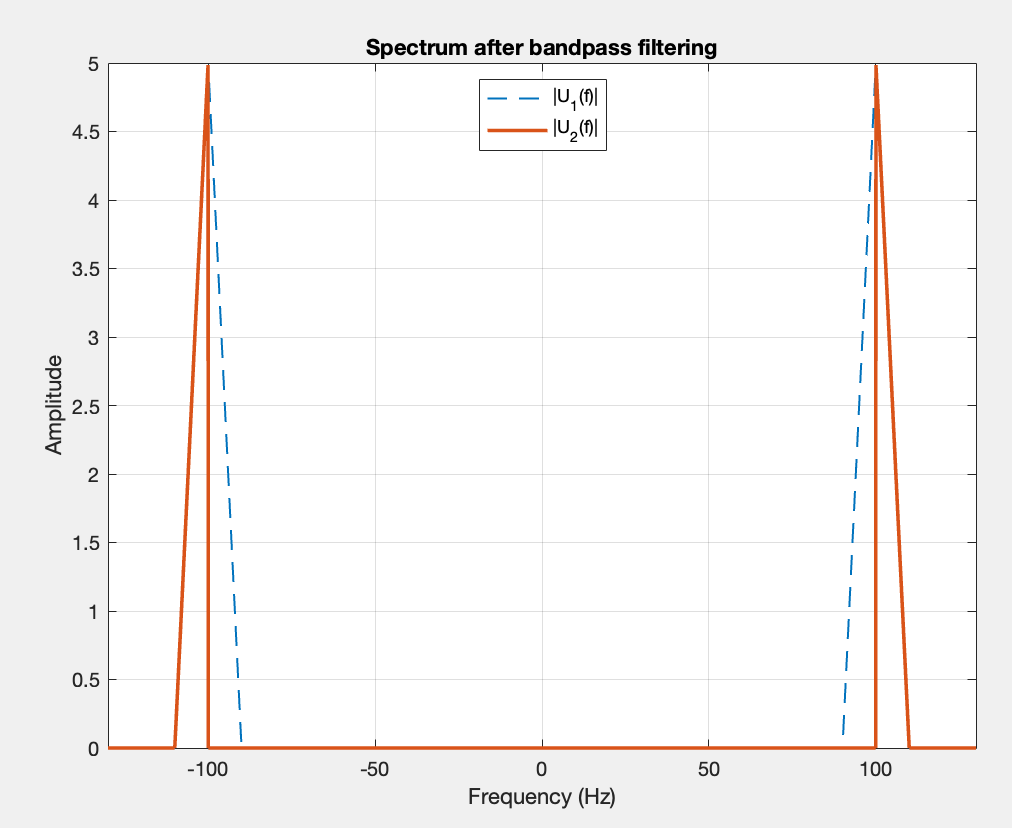
\includegraphics[width=0.6\linewidth]{image/question2.png}
    \caption{Magnitude spectra $|U_1(f)|$ and $|U_2(f)|$; the filter preserves only the upper sideband around $\pm 105$ Hz.}\label{fig:q2}
\end{figure}

\item[(b)] Let $f_c = 100$ Hz. Removing the lower sideband leaves the complex envelope
\[
s(t) = \int_0^{10} (10-\nu) e^{j 2\pi \nu t}\, d\nu
      = \frac{1-e^{j20\pi t}}{\bigl(2\pi t\bigr)^2} + j\,\frac{5}{\pi t},\ % chktex 3
\]
with finite limits $s(0)=50$ and $s'(0)=0$. Therefore
\[
u_2(t) = u_c(t) \cos(2\pi f_c t) - u_s(t) \sin(2\pi f_c t),
\quad
u_c(t)=\frac{1-\cos(20\pi t)}{4\pi^2 t^2},\quad
u_s(t)=\frac{5}{\pi t} - \frac{\sin(20\pi t)}{4\pi^2 t^2},
\]
with $u_c(0)=50$ and $u_s(0)=0$ understood by continuity.

\item[(c)] Yes. Because $H(f)$ passes only the upper sideband of the original DSB-SC spectrum, the complex envelope $s(t)=u_c(t)+j u_s(t)$ contains only nonnegative baseband frequencies ($\nu \ge 0$). Consequently, $u_s(t)$ is the Hilbert transform of $u_c(t)$, which is characteristic of single-sideband AM signals obtained from analytic (positive-frequency) spectra.
\end{enumerate}

\end{document}
